% Paper 2015
\documentclass[11pt,a4paper]{IEEEtran}

\usepackage{ifpdf}
\usepackage{cite}

\ifCLASSINFOpdf
    \usepackage[pdftex]{graphicx}
    \graphicspath{{../pdf/}{../jpeg/}}
    \DeclareGraphicsExtensions{.pdf,.jpeg,.png}
\else
    \usepackage[dvips]{graphicx}
    \graphicspath{{../eps/}}
    \DeclareGraphicsExtensions{.eps}
\fi

\usepackage[cmex10]{amsmath}

\usepackage{array}
\usepackage{fixltx2e}

\ifCLASSOPTIONcaptionsoff
  \usepackage[nomarkers]{endfloat}
 \let\MYoriglatexcaption\caption
\renewcommand{\caption}[2][\relax]{\MYoriglatexcaption[#2]{#2}}
\fi

\usepackage{url}

\usepackage{siunitx}
\DeclareSIUnit\photon{\ensuremath{\gamma}}
\DeclareSIUnit\proton{p}
\DeclareSIUnit\neutron{n}

\usepackage{booktabs}

\usepackage{graphicx}
\usepackage{epstopdf}

\usepackage{caption}
\usepackage{subcaption}

\usepackage{todo}
%\renewcommand\todo[1]{\relax}
%\renewcommand\todos{\relax}

\usepackage{bpchem}
\def\U238{\BPChem{\^{238}U}}

% correct bad hyphenation here
\hyphenation{op-tical net-works semi-conduc-tor}

\begin{document}

\title{
    Detailed Geant4 simulations of the ANITA and ANITA-CUP neutron facilities
}

\author{%
    Q. Hong,
    S. P. Platt,
    A. V. Prokofiev,
    E. Passoth
    \thanks{%
        Qian Hong and Simon Platt are with the University of Central Lancashire, England. Alexander Prokofiev and Elke Passoth are with the The Svedberg Laboratory, University of Uppsala, Sweden.
    }
}

\maketitle

\begin{abstract}
    Monte Carlo simulation of spallation neutron source of ANITA at TSL was used to analyze radiation fields at the Close User Position (CUP) and Standard User Position(SUP) for single-event effect testing. ...
    \todo{Revise abstract}
\end{abstract}

\section{Introduction}
\todo{Review introduction}
\IEEEPARstart{M}{onte} Carlo simulations of naked spallation neutron sources at Los Alamos Neutron Science Center (LANSCE) Weapons Neutron Research (WNR) Target 4\cite{Wender87} and the ANITA beam at the University of Uppsala The Svedberg Laboratory (TSL) have been completed using Geant4 and proved that Binary intranuclear cascade (INC) model gave a good representation of neutron spectra than Bertini INC model did\cite{Platt13}. Simulation result of neutron spectra using Geant4 with Binary INC model is below measurement data from ANITA neutron facility. It is likely to be influenced by our omission of collimator, shielding, and bending magnet component. This work is to verify this hypothesis is correct. In addition, we are intested in the gamma field at CUP and SUP in spallation neutron source at the ANITA neutron facility at TSL for SEE testing.

\section{Modelling}
Simulations were conducted using Geant4 version 10.0 and the binary intranuclear cascade model, as recommended in~\cite{Platt13}.
A detailed model of the ANITA geometry was implemented in Geant4, as illustrated in Fig.~\ref{fig:ANITAoverview}
Description of the geometry is given in \cite{Prokofiev2009,Prokofiev14}.
%; a summary only is given here.
%The spallation target is a tungsten cylinder of diameter \SI{5}{\cm} and length \SI{2.4}{\cm}~\cite{ANITAdrawing}.
%The target is cooled by water and surrounded by a stainless-steel cooling jacket.
%The target assembly with its cooling jacket appears as a small blue rectangle in Fig.~\ref{fig:ANITAoverview}.
%Lead shielding blocks in the target region are also modelled, and shown in red Fig.~\ref{fig:ANITAoverview}.
%A large electromagnet surrounding the target is modelled and shown in Fig.~\ref{fig:ANITAoverview} in grey (iron) and yellow (copper).
%An iron collimator with variable apertures is modelled  and shown downstream of the target (grey).
Except where indicated otherwise, all results in this summary are for the standard collimator size (\SI{10.2}{\cm} diameter).
In the final paper we will present results for cylindrical collimators in the range from \SIrange{3}{30}{\cm} diameter.
Simulated protons were incident axially at an energy of \SI{180}{\MeV}.
Resulting gamma and neutron fields were evaluated at several detector locations.
In this paper results are presented for three of these: the Standard User Position (SUP), \SI{2.5}{\m} downstream of the target~\cite{Prokofiev2009}, the Close User Position (CUP), \SI{0.75}{\m} downstream of the target, and the CUP-TOF, \SI{0.84}{m} downstream of the target.
%N.B. This is downstream of the downstream edge of the target in Qian's model.
The SUP and CUP positions are of interest as they are positions used for SEE tests; the CUP-TOF position is the location of thin-film breakdown counter (TFBC) detectors used for beam monitoring and characterisation using time-of-flight (TOF) techniques.
Model validation will be demonstrated against CUP-TOF data (section~\ref{tbd}).

\begin{figure}[t]
	\centering
	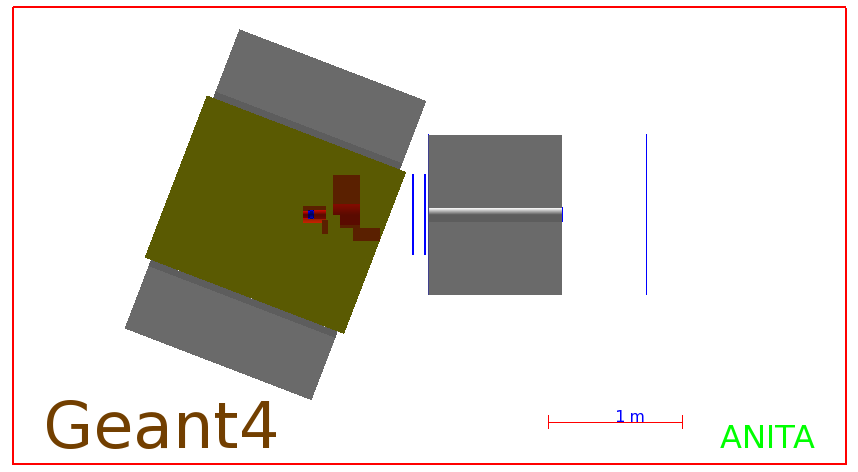
\includegraphics[width=\columnwidth]{overview.png}
	\caption{
        Simulated ANITA facility overview seen from above (yellow: bending magnet; red: shielding components; blue: target cooling jacket (enclosing the target); grey: collimator; blue: detector system)
    }
	\label{fig:ANITAoverview}
\end{figure}

\section{Results}
In previous work Platt et al.~\cite{Platt13} reported simulations of a naked ANITA target, demonstrating good qualitative agreement with independent calculations and measurements of the fast neutron field at ANITA SUP~\cite{Prokofiev2009}.
Part of the motivation for this work was to investigate whether improvements in the fidelity of the geometry used in the Geant4 model would lead to increased quantitative agreement.
\todo{Review first part of Results section -- move to introduction?}

\subsection{Neutrons}
Fig.~\ref{fig:SUPDensity} shows neutron spatial distribution at the SUP, for neutrons above \SI{10}{\MeV}.
The collimation effect is clearly visible.
Within the beam umbra the predicted neutron fluence rate above \SI{10}{\MeV} at a proton current of \SI{200}{\nA} is \SI{7.1e5}{\neutron\per\cm\squared\per\second}, compared to \SI{5.7e5}{\neutron\per\cm\squared\per\second} from earlier calculations~\cite{Platt13} and \SI{9.3e5}{\neutron\per\cm\squared\per\second} from the standard facility parameterisation~\cite{Prokofiev2009}.
The parameterisation therefore exceeds the present calculations by 31\%.

\begin{figure}[t]
    \begin{minipage}{\columnwidth}
        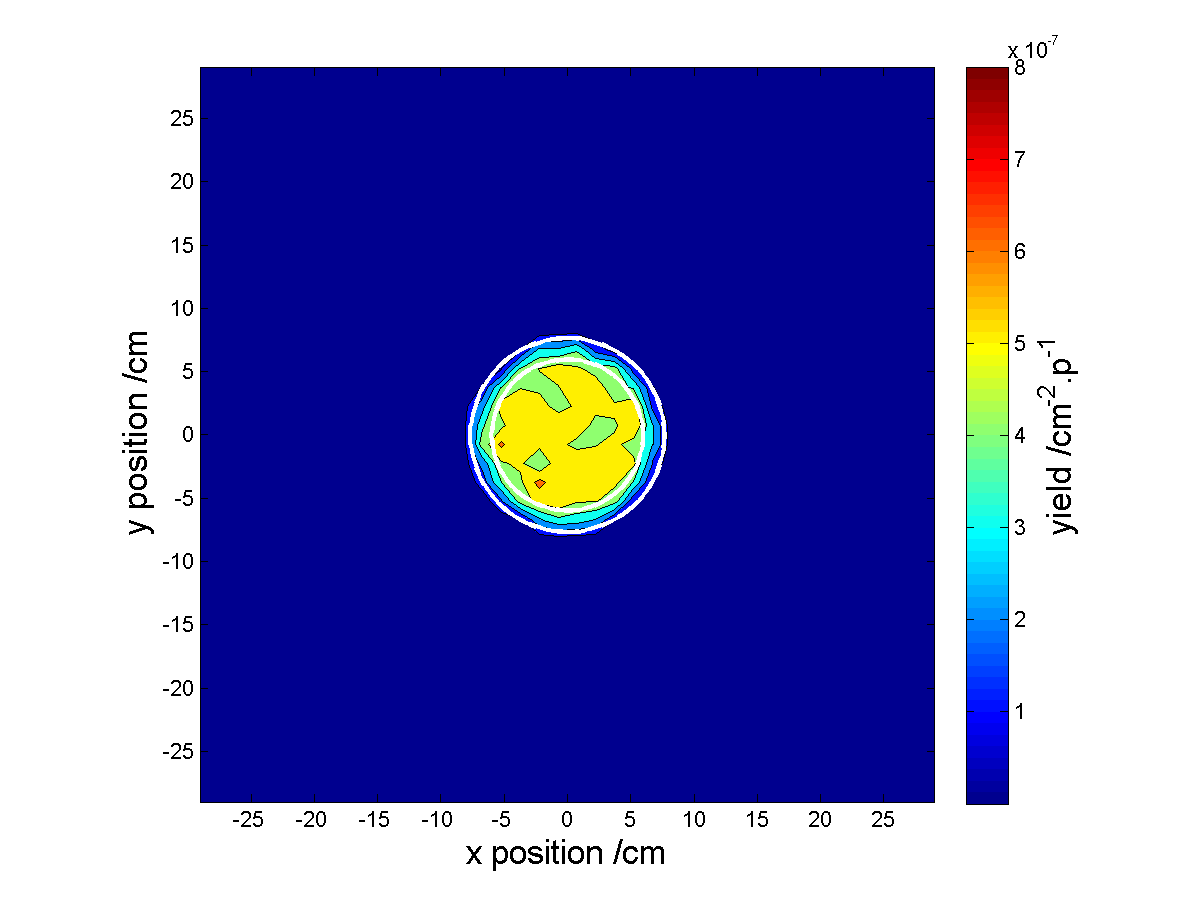
\includegraphics[width=\columnwidth]{SUP10ColSpatialDistribution10MeVRADECS.png}
        \subcaption{
            Standard User Position.
            Concentric white circles indicate nominal umbra and penumbra limits.
        }
        \label{fig:SUPDensity}
    \end{minipage}
    \begin{minipage}{\columnwidth}
        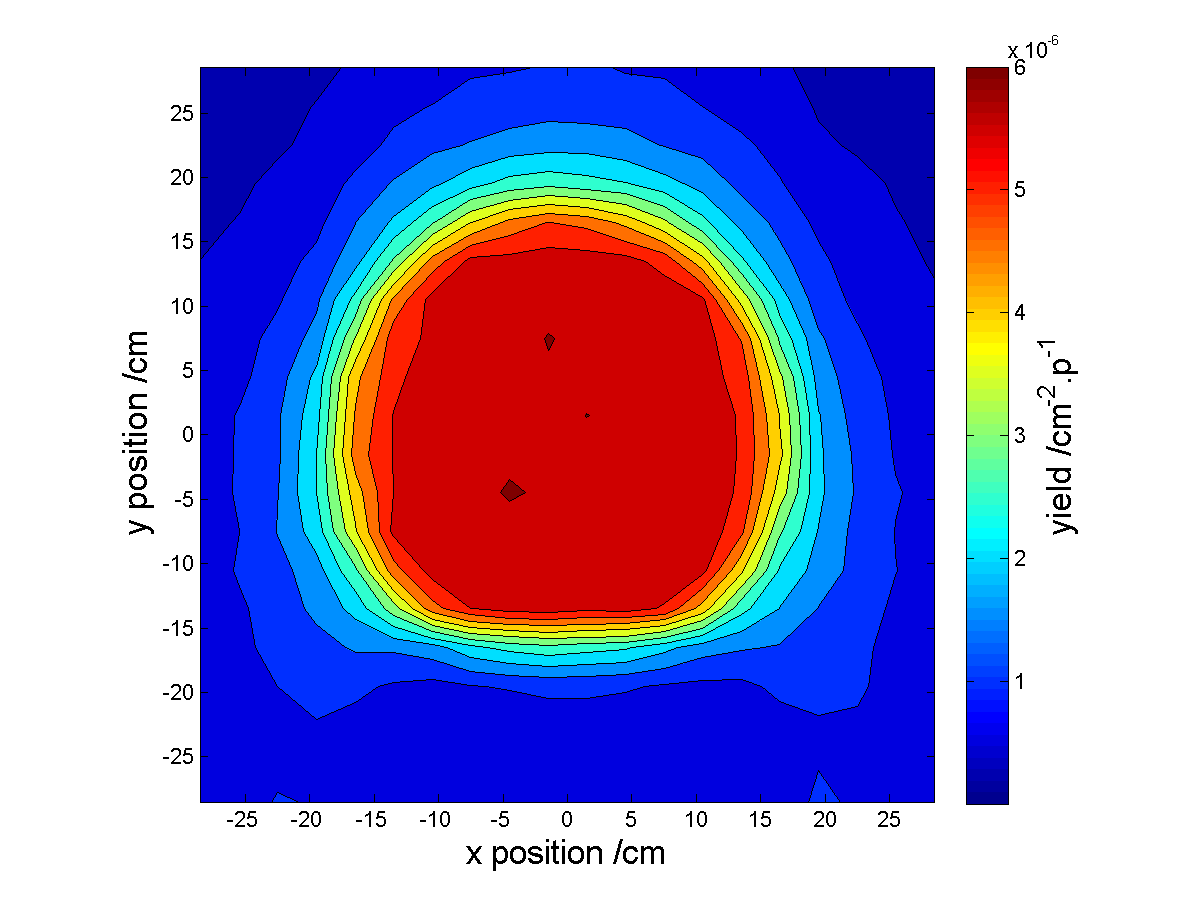
\includegraphics[width=\columnwidth]{CUP10ColSpatialDistribution10MeV.png}
        \subcaption{Close User Position}
        \label{fig:CUPDensity}
    \end{minipage}
    \caption{
        Spatial distribution of neutrons above \SI{10}{\MeV} at SUP and CUP.
        \SI{10.2}{\cm} diameter collimator.
    }
\end{figure}

Fig.~\ref{fig:CUPDensity} shows equivalent data for the CUP.
In the central region the predicted neutron fluence rate above \SI{10}{\MeV} at a proton current of \SI{200}{\nA} is \SI{0}{\neutron\per\cm\squared\per\second}, compared to \SI{0}{\neutron\per\cm\squared\per\second} from the standard facility parameterisation~\cite{Prokofiev14}.
The parameterisation therefore exceeds the present calculations about TBD\%.
\todo{Complete quantification at CUP}.
The results show\ldots
\todo{Describe the results: contours and profile at CUP and SUP}

Neutron beam monitoring and characterisation at TSL includes measurements with \U238\ TFBCs~\cite{Prokofiev14}.
Fig.~\ref{fig:CUPProfile} shows neutron fluence profile at the CUP, compared with measurements~\cite{Prokofiev14}.
In Fig.~\ref{fig:CUPProfile} simulated data were folded in energy with the neutron fission cross section for \U238~\cite{tbd}.
The results show\ldots
\todo{Describe the results: contours and profile at CUP}

\begin{figure}[t]
    \centering
    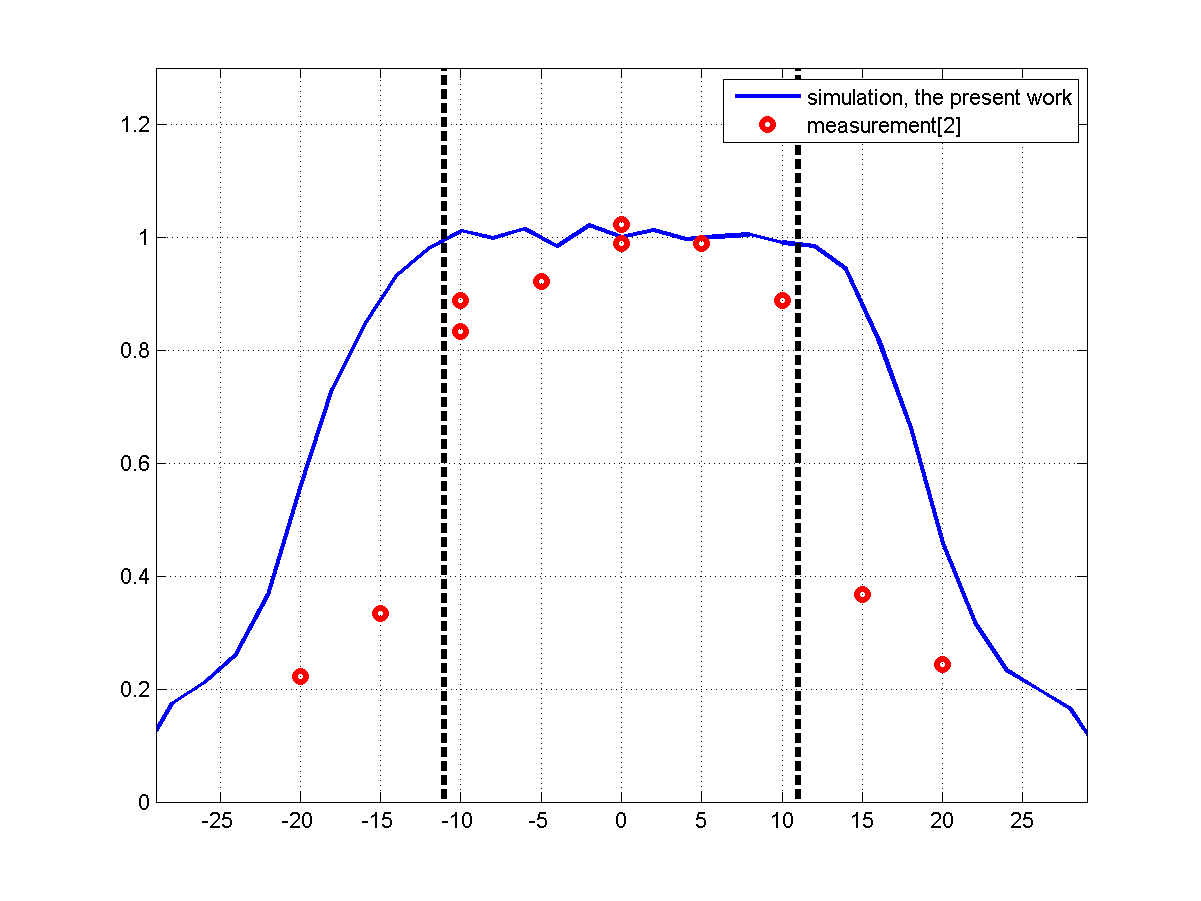
\includegraphics[width=\columnwidth]{CUPTOF10beamproRADECS.png}
    \caption{
        Neutron profile at the CUP, normalised to fluence rate on axis.
        \SI{10.2}{\cm} collimator}
    \label{fig:CUPProfile}
\end{figure}

Fig.~\ref{fig:TOFSpectra} compares simulated and measured TOF spectra at the CUP-TOF position.
Neutron time of flight data from the simulation were folded in energy with the \U238\ fission cross-section, convolved with a \SI{5}{\ns} rectangle function approximating the primary proton micropulse shape, and overlapped at \SI{45}{\ns}, representing the timing ambiguity due to the micropulse period.
The results show\ldots
\todo{Explain what the results show.}

\begin{figure}[t]
    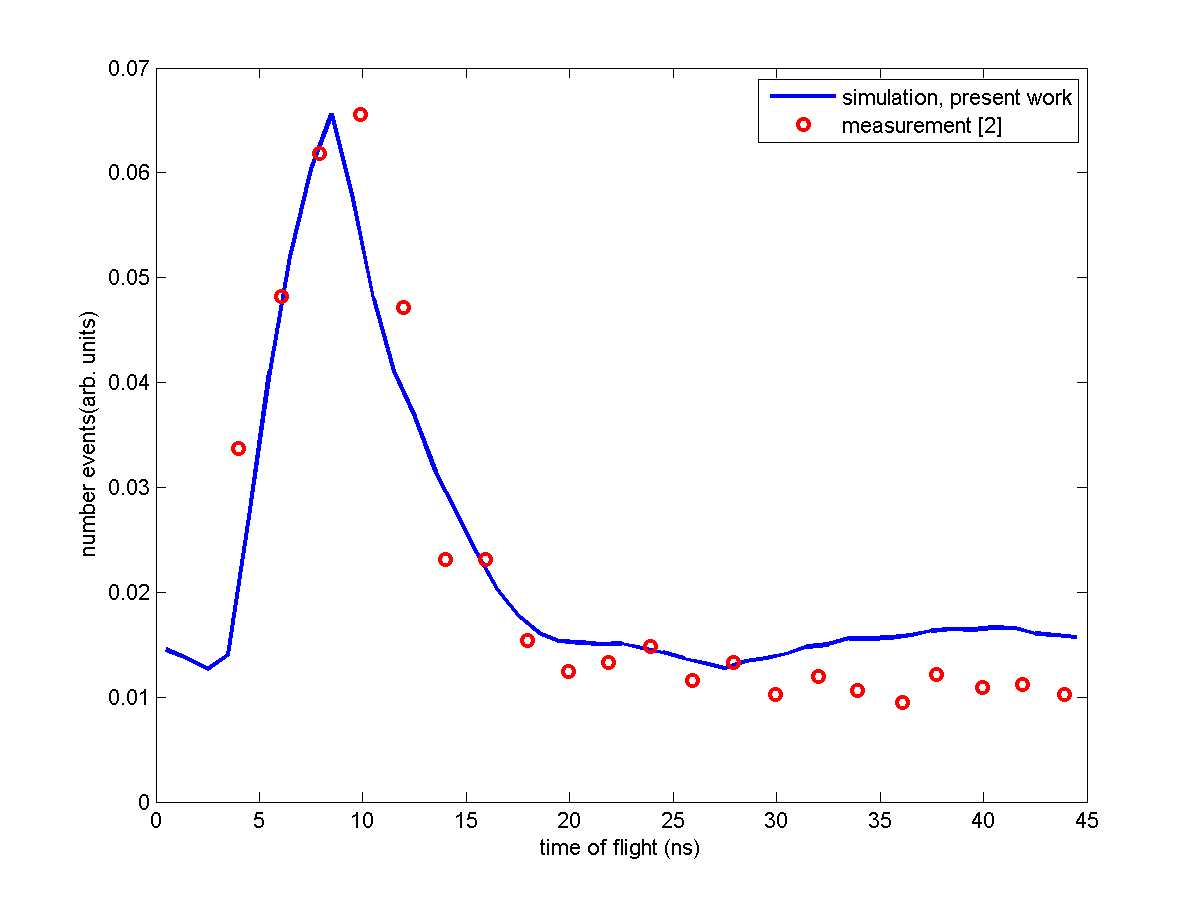
\includegraphics[width=\columnwidth]{CUPTOFtofspectraRADECS.png}
    \caption{
        Neutron time of flight spectra at the CUP-TOF position, with \SI{3}{\cm} collimator
        }
    \label{fig:TOFSpectra}
\end{figure}




Fig.~\ref{fig:Lethargyplots} compares calculates spectra at SUP and CUP with their respective standard facility models~\cite{Prokofiev2009,Prokofiev14}.
The SUP data are also compared with results from preliminary Geant4 simulations~\cite{Platt13}.
The results show\ldots
\todo{Describe the neutron spectra.}

\begin{figure}[t]
    \begin{minipage}{\columnwidth}
        \centering
        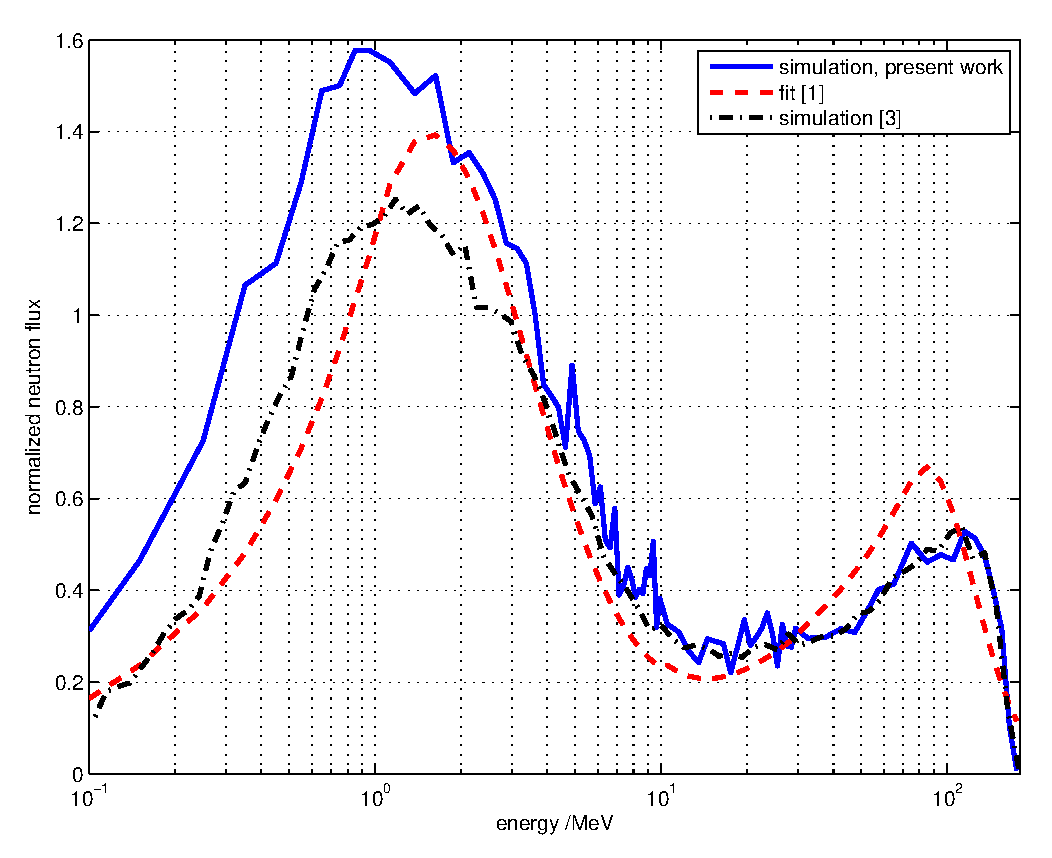
\includegraphics[width=0.9\columnwidth]{SUPNormalisedRADECS.eps}
        \subcaption{
            SUP.
            The comparison is against preliminary Geant4 modelling with a naked target model~\cite{Platt13} and against the standard facility parameterisation~\cite{Prokofiev2009}
        }
    \end{minipage}
    \begin{minipage}{\columnwidth}
        \centering
        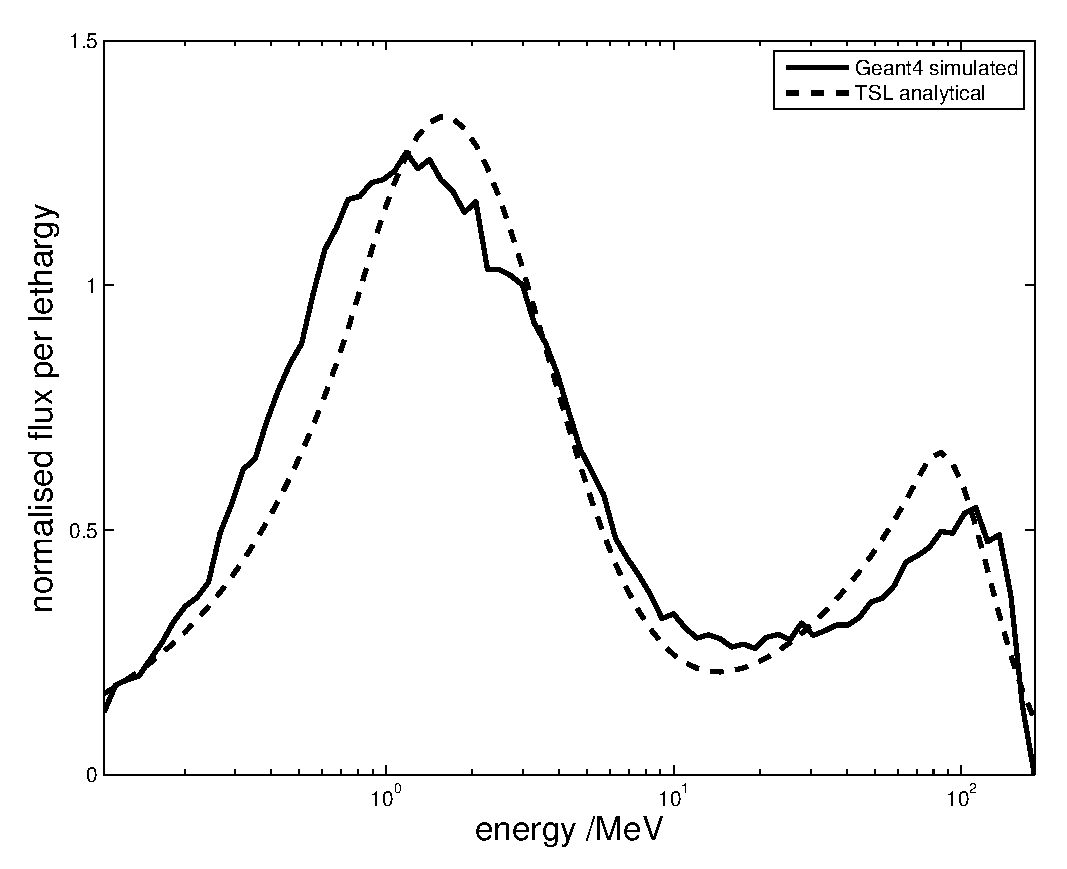
\includegraphics[width=0.9\columnwidth]{ANITALetYieldnormalisedRADECS.eps}
        \subcaption{
            CUP.
            The comparison is against the standard facility parameterisation~\cite{Prokofiev2009}
        }
    \end{minipage}
	\caption{
        Calculated neutron spectra, normalised to fluence above \SI{10}{\MeV}.
        \SI{10.2}{\cm} collimator
    }
	\label{fig:Lethargyplots}
\end{figure}

Fig.~\ref{fig:DifferentialSpectra} summarise neutron yield results by comparing differential flux as calculated in this work with facility parameterisations~\cite{Prokofiev2009,Prokofiev14}.
The SUP calculations and parameterisations agree very closely below \SI{20}{\MeV}; the parameterisation exceeds the calculations somewhat above that energy.
At CUP the parameterisation exceeds the Geant4 calculations by about TBD\% below \SI{20}{\MeV} and slightly more above that energy.
\todo{Improve precision of the summary description of differential spectra.}

\begin{figure}[t]
    \centering
    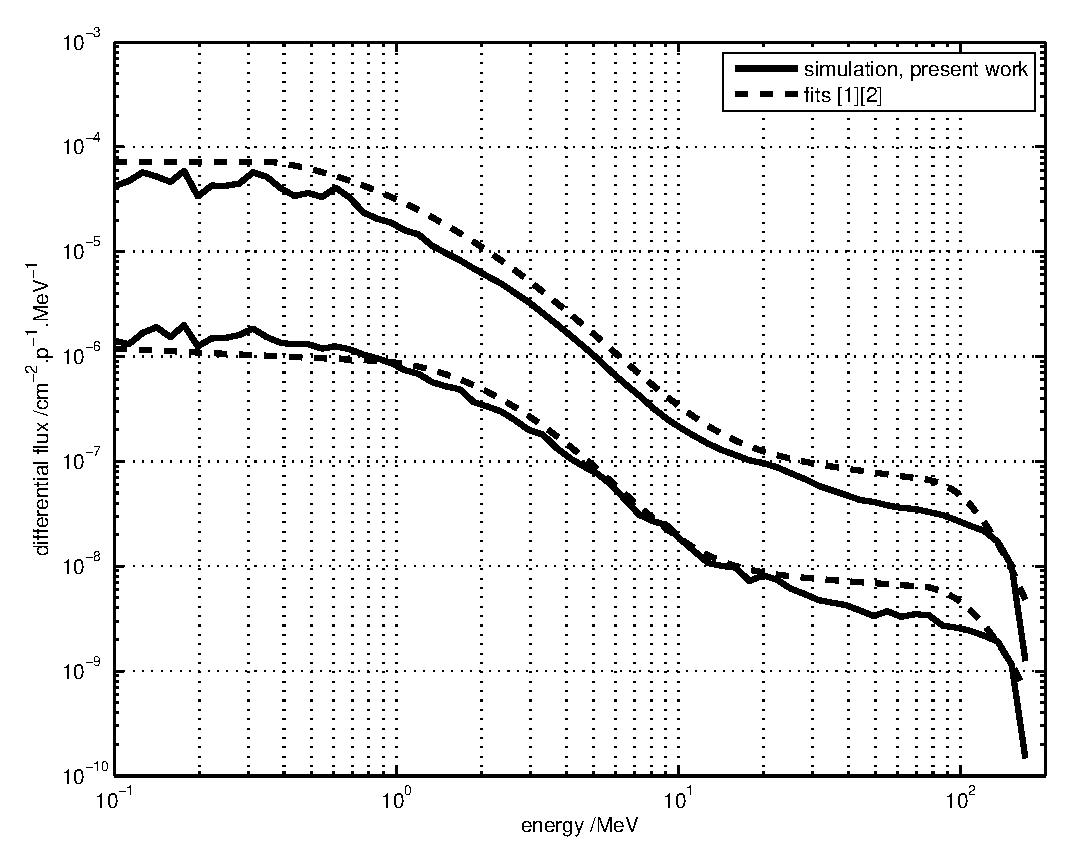
\includegraphics[width=0.9\columnwidth]{DiffYieldComparedSUPCUP10.eps}
    \caption{
        Differential neutron spectra at CUP and SUP (\SI{10.2}{\cm} collimator), comparing results of this work to facility parameterisations~\cite{Prokofiev2009,Prokofiev14}
    }
    \label{fig:DifferentialSpectra}
\end{figure}




\subsection{Photons}
Fig.~\ref{fig:GammaSpatialDistribution} shows the calculated spatial distribution of gamma photons at SUP and CUP.
Fig.~\ref{fig:DifferentialGammaSpectra} shows the calculated differential gamma spectra within the central region of the spatial distribution.
The results show\ldots
\todo{Describe the gamma results}

\begin{figure}[t]
    \begin{minipage}{\columnwidth}
        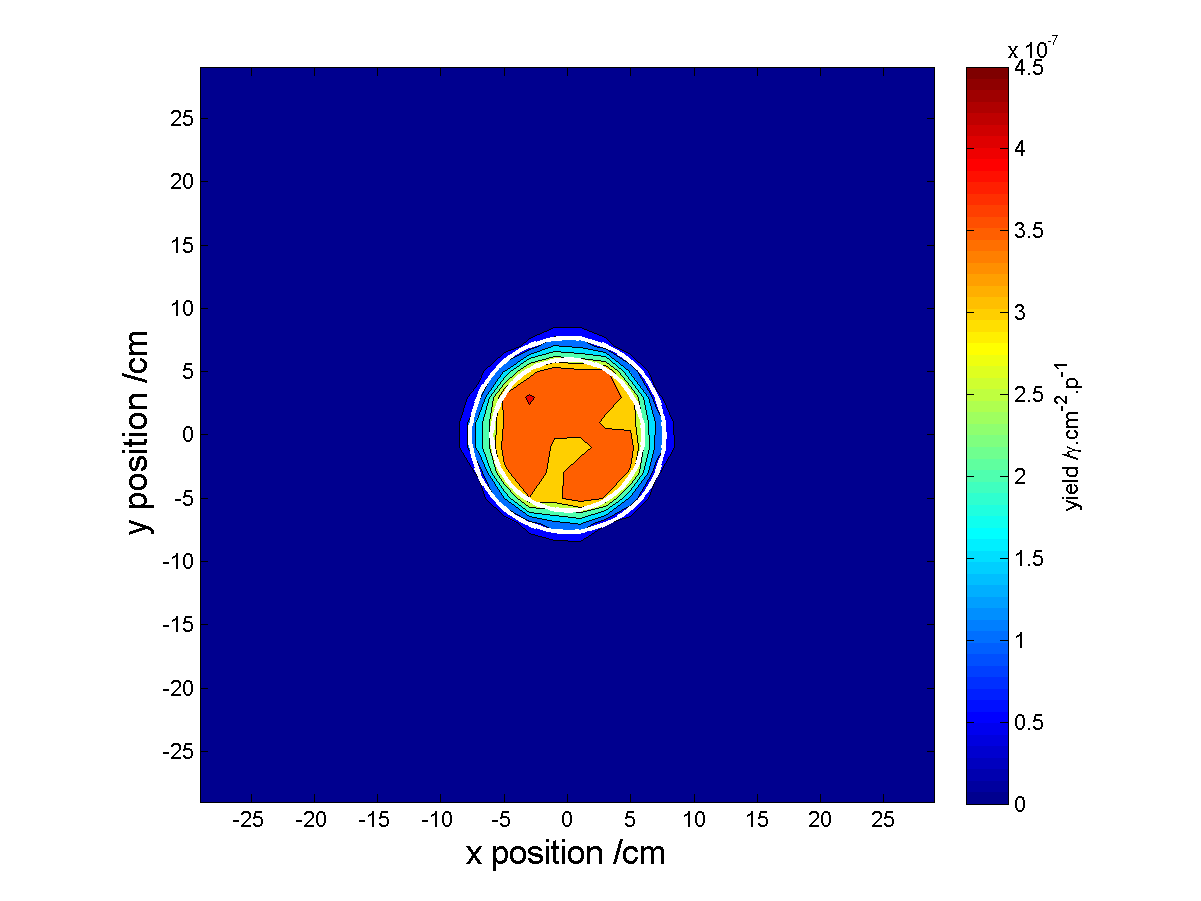
\includegraphics[width=\columnwidth]{SUP10ColSpatialDistributionAllG.png}
        \subcaption{Standard User Position}
        \label{fig:GammaSpatialDistributionSUP}
    \end{minipage}
    \begin{minipage}{\columnwidth}
        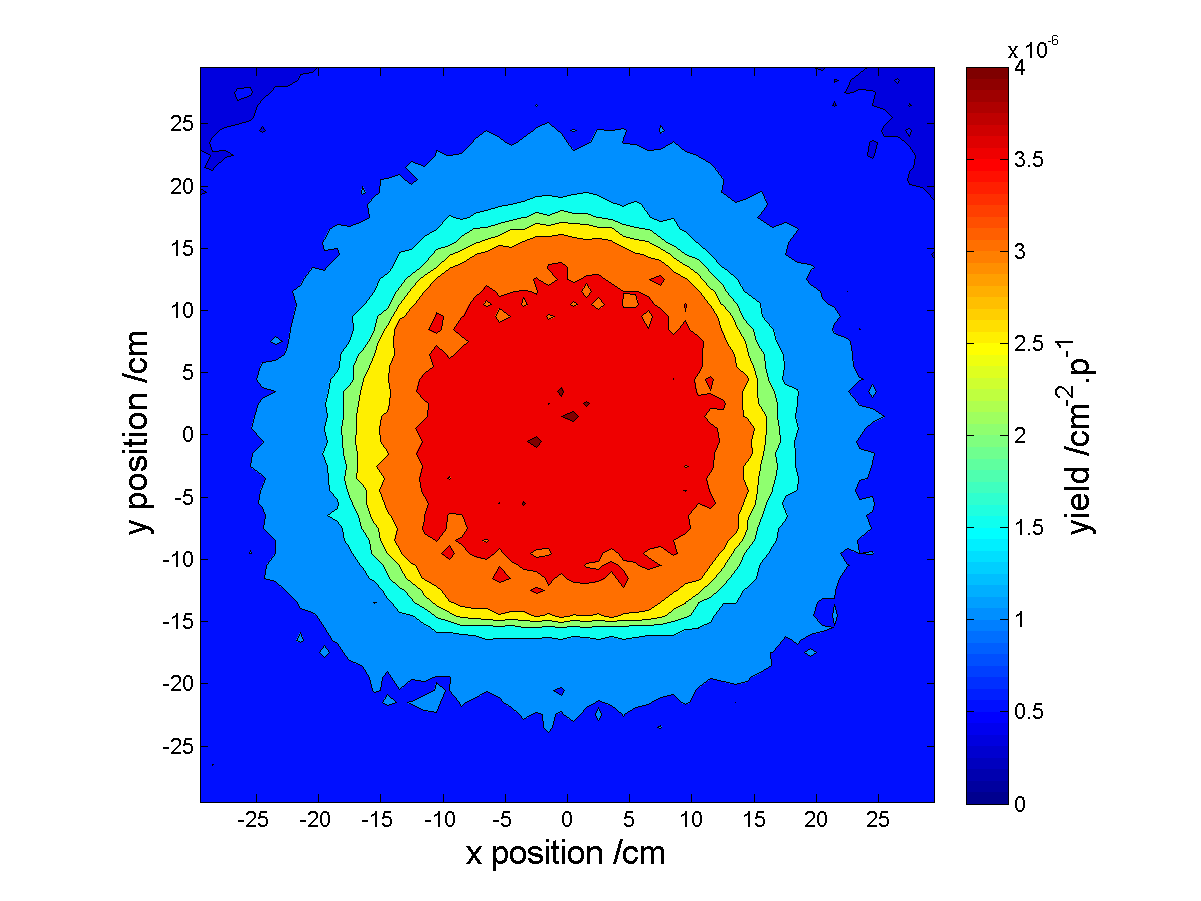
\includegraphics[width=\columnwidth]{CUP10ColSpatialDistributionAllG.png}
        \subcaption{Close User Position}
        \label{fig:GammaSpatialDistributionCUP}
    \end{minipage}
    \caption{
        Calculated gamma spatial distribution.
        \SI{10.2}{\cm}collimator
    }
    \todo{It would be better if gamma spatial distribution were expressed as dose, rather than number of photons. Not in time for the abstract submission, however!}
    \label{fig:GammaSpatialDistribution}
\end{figure}

\begin{figure}[t]
    \centering
    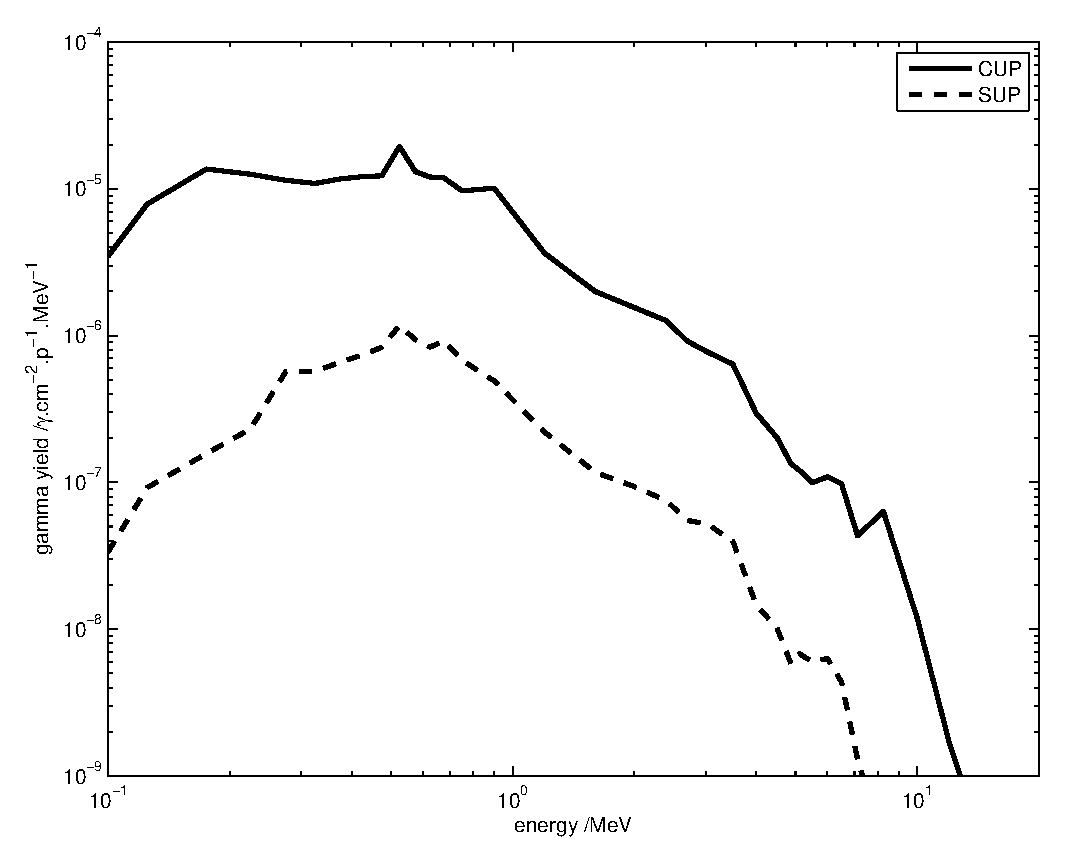
\includegraphics[width=0.9\columnwidth]{gDYieldcomparedRADECS.eps}
    \caption{
        Calculated gamma spectra at CUP and SUP.
        \SI{10.2}{\cm} collimator
    }
    \label{fig:DifferentialGammaSpectra}
\end{figure}

Fig.~\ref{fig:GammaDoseEnergy} shows the calculated distribution of gamma dose, obtained by folding the gamma spectra (Fig~\ref{fig:GammaDoseEnergy}) with dose conversion data from \cite{tbd}.
The results show\ldots
\todo{Describe the gamma dose versus energy graphs.}
The calculated dose rate at \SI{200}{\nA} primary proton current is \SI{21}{\milli\gray\per\hour} at SUP and \SI{370}{\milli\gray\per\hour} at CUP.
\todo{Discuss calculated dose rates}

\begin{figure}[t]
    \begin{minipage}{\columnwidth}
        \centering
        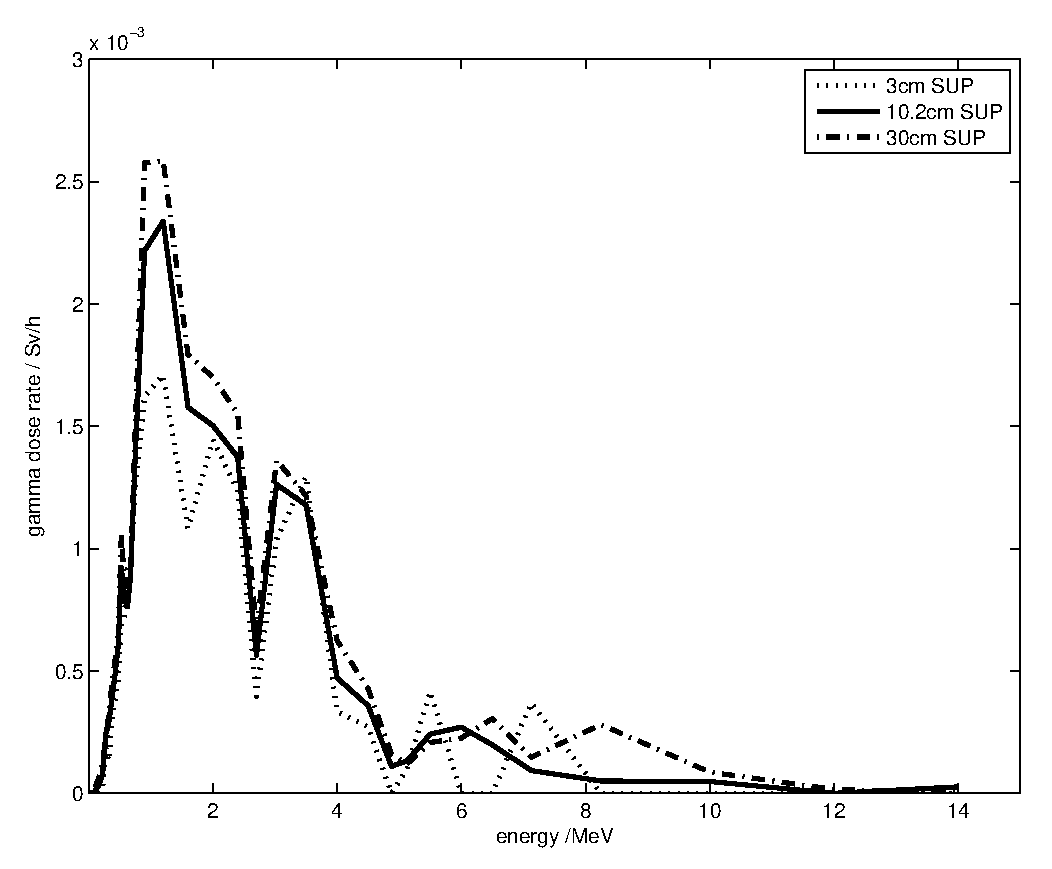
\includegraphics[width=0.9\columnwidth]{DoseVSenergySUP.eps}
        \subcaption{Standard User Position}
        \label{fig:GammaDoseEnergySUP}
    \end{minipage}
    \begin{minipage}{\columnwidth}
        \centering
        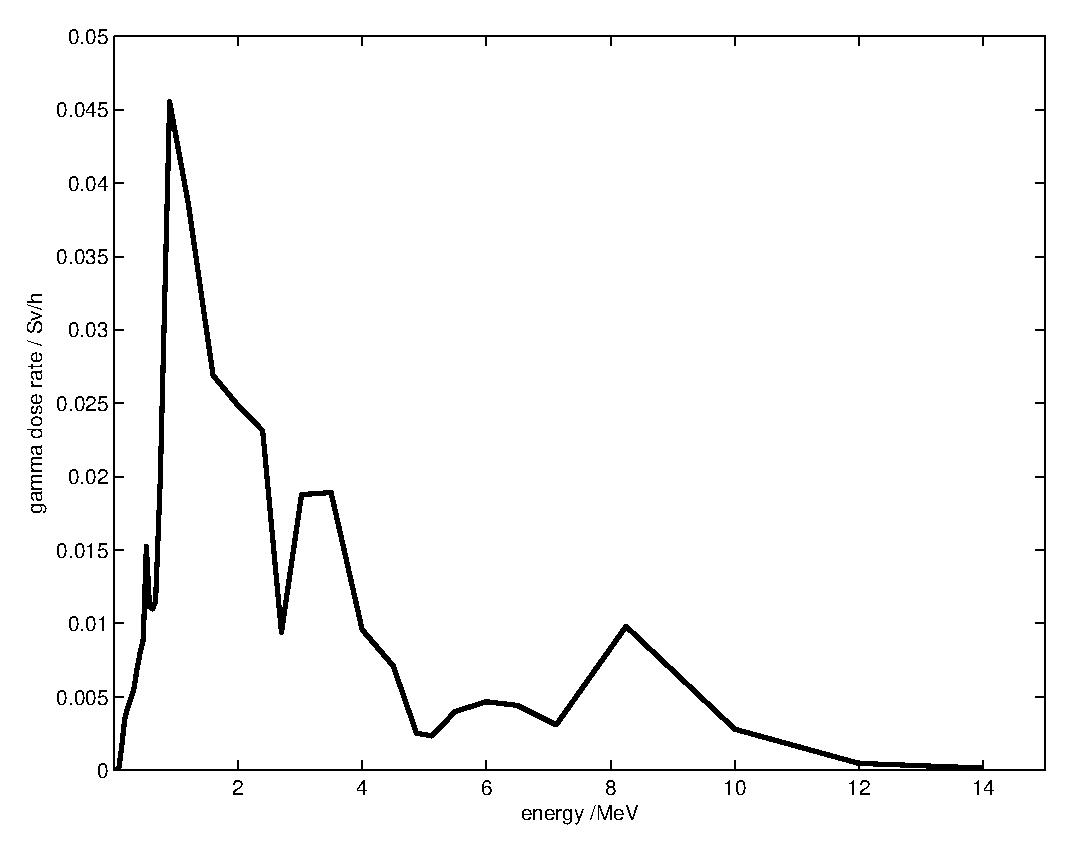
\includegraphics[width=0.9\columnwidth]{DoseVSenergyCUP.eps}
        \subcaption{Close User Position}
        \label{fig:GammaDoseEnergyCUP}
    \end{minipage}
    \caption{
        Calculated gamma dose spectra.
        \SI{10.2}{\cm} collimator
    }
    \label{fig:GammaDoseEnergy}
\end{figure}

\section{Discussion}
\todo{Discussion}

\todo{Complete citations}

\begin{thebibliography}{99} % Bibliography - this is intentionally simple in this template

\bibitem{Wender87}
S.A. Wender and P.W. Lisowski,
\newblock A white neutron source from 1 to 400 MeV,										% title	
\newblock {\em Nucl. Instr. Meth. Phys. Res. B}, vol. 24-25, pp. 897-900.					% vol:page, 2011

\bibitem{Platt13}
Platt, S.P. and Hong, Q. and Mein, S.J. and Zhang, L.H.,
\newblock Neutron and gamma fields at neutron spallation sources for single-event-effects testing,		% title	
\newblock {\em in Proc. 14th European Conf. Radiat. Effects Compon. Syst. 2013,} pp 1-4			% vol:page, 2011

\bibitem{Prokofiev14}
Prokofiev, A.V. and Blomgren, J. and Majerle, M. and Nolte, R. and Rottger, S. and Platt, S.P. and Cai Xiao Xiao and Smirnov, A.N.,
\newblock Characterization of the ANITA Neutron Source for Accelerated SEE Testing at the Svedberg Laboratory,		% title	
\newblock {\em in Proc. IEEE Radiation Effects Data Workshop. 2009,} pp 166-173 									% vol:page, 2011

\bibitem{Prokofiev2009}
Prokofiev, A.V. and Passoth, E. and Hjalmarsson, A. and Majerle, M.,
\newblock CUP-A New High-Flux Irradiation Position at the ANITA Neutron Facility at TSL,		% title	
\newblock {\em in Proc. IEEE Trans. Nucl. Sci. 2014}, pp 1929-1936 							% vol:page, 2011

\bibitem{ANITAdrawing}
Prokofiev, A.V.
\newblock personal communication
\newblock {\em TSL, Sep. 2013}

\end{thebibliography}

\cleardoublepage

\todos

\end{document} 